\subsection{Results and conclusions of the exosystem control design}
\label{Exo_result}

As can be seen in \figref{fig:sin_disturbance}, by applying the disturbance through an exosystem as an input to the original system, the slowly-varying sinusoidal appears on the output.

\begin{figure}[H]
\centering
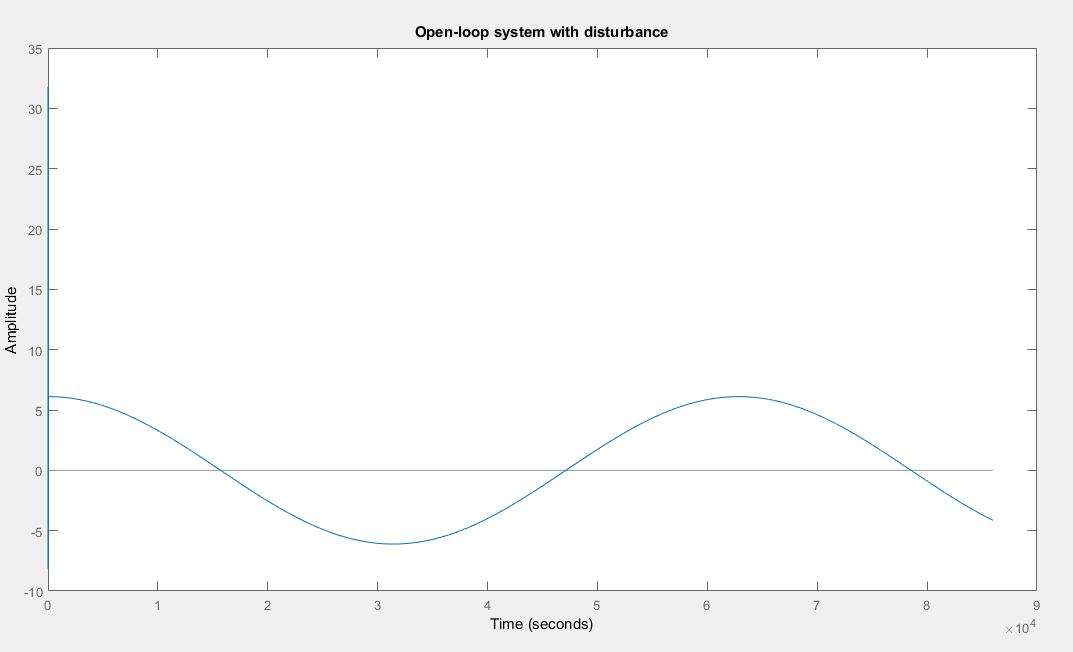
\includegraphics[width=1.1\textwidth]{rapport/billeder/temporary/sinusdist}
\caption{Slowly varying sinusoidal disturbance on the output.}
\label{fig:sin_disturbance}
\end{figure}

However, during the real-life measurements and according to the simulation of the genset, this result could never be obtained. The main reason why this result could not be achieved is that the genset with its inner AVR control can easily react to small and slow changes on the voltage, therefore would the disturbance all ready be handled by the genset and not be present on the output. 

In simulation where the genset is unable to handle the disturbance, applying the designed controller, results in the following dynamics for disturbance rejection, that are shown in \figref{fig:sin_disturbance_reject} where it is seen that the disturbance is effectively rejected. 

\begin{figure}[H]
\centering
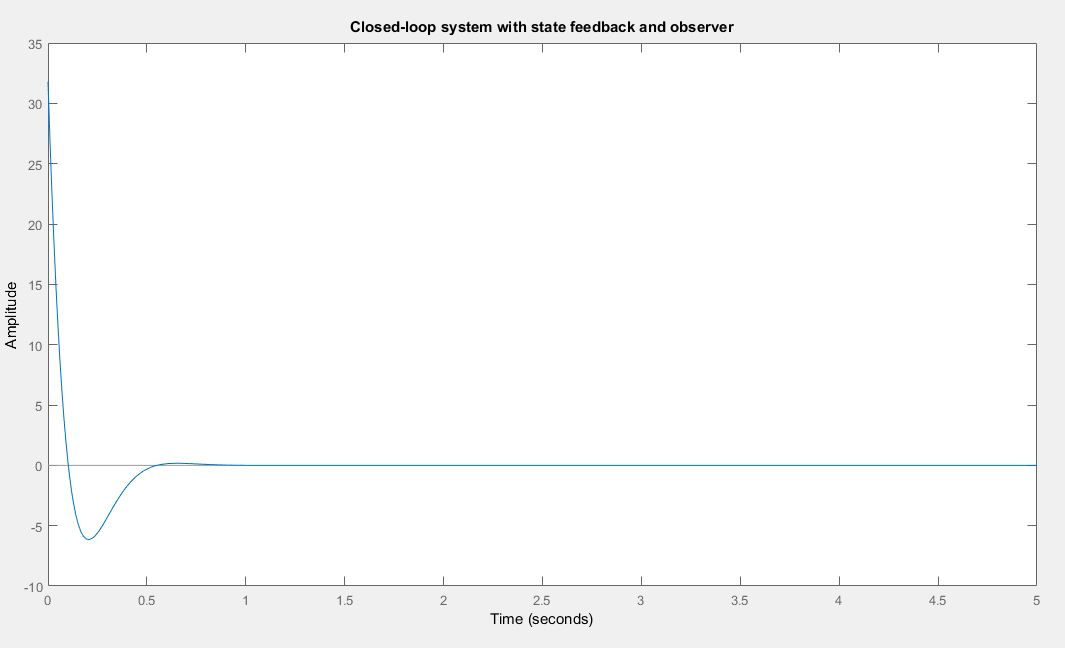
\includegraphics[width=1.1\textwidth]{rapport/billeder/temporary/eliminated_disturbance}
\caption{Sinusoidal disturbance rejected due to observer, feedback and state space control.}
\label{fig:sin_disturbance_reject}
\end{figure}

After coming to the realization that this approach does not fit reality, it was decided to put more focus on the fast varying load and make a design that can handle it in simulation and in reality. Therefore the following sections deals with a more suitable controller design. 